\documentclass[10pt,twocolumn]{article}

\usepackage[utf8]{inputenc}
\usepackage[T1]{fontenc}
\usepackage[spanish,es-noquoting]{babel}
\usepackage{lmodern}
\usepackage{amsmath,amssymb}
\usepackage{graphicx}
\usepackage{booktabs}
\usepackage{multirow}
\usepackage{array}
\usepackage{float}
\usepackage{hyperref}
\usepackage{caption}
\usepackage{geometry}
\usepackage{enumitem}
\usepackage{xcolor}

\geometry{margin=1.8cm}
\setlength{\columnsep}{0.7cm}
\setlength{\textfloatsep}{8pt}
\setlength{\floatsep}{6pt}
\setlength{\intextsep}{6pt}
\captionsetup{font=small, skip=4pt}
\hypersetup{
    colorlinks=true,
    linkcolor=blue,
    urlcolor=blue,
    citecolor=blue
}

\title{\textbf{Práctica Final: SAC para manipulación robotica\\
en control continuo}}
\author{Antonio Lorenzo \and Andrés Martínez \and Pablo García Molina}
\date{Curso 2025/2026}

\begin{document}

\twocolumn[
\maketitle
\begin{abstract}
En esta práctica se estudia el uso del algoritmo Soft Actor-Critic (SAC) en tareas de manipulación robótica simuladas dentro del entorno \texttt{Pusher-v5}. Se analiza su rendimiento y la influencia de distintos hiperparámetros en la estabilidad del aprendizaje.

Los resultados muestran que el uso exclusivo de observaciones visuales no es suficiente para aprender políticas estables, mientras que la combinación con información tabular mejora claramente el rendimiento. Además, SAC resulta robusto, pero sensible a la elección de hiperparámetros como la tasa de aprendizaje o la resolución de entrada.

Por último, se observa la importancia de la alineación entre la función de recompensa utilizada durante el entrenamiento y la métrica de evaluación final.

Código disponible en: \url{https://github.com/andresmartinezfuentes/pusher-v5}
\end{abstract}
\vspace{0.2cm}
]

\section{Introducción}

El entorno \texttt{Pusher-v5} que se caracteriza por ser un entorno de manipulación robótica en simulación física, donde el objetivo del agente es controlar un brazo robótico para empujar un objeto hasta una posición objetivo sobre una superficie plana. A diferencia de los entornos de locomoción, no hay un final del episodio claro donde el agente se cae o se coloca en un ángulo no sano, sino que el final del episodio se determina al cabo de 100 \texttt{steps}. El agente opera en un espacio de acciones continuo, típicamente aplicando torques a las articulaciones del brazo. La función de recompensa combina la distancia entre el objeto y el objetivo, así como la distancia entre el actuador final y el objeto, premiando comportamientos coordinados de aproximación y empuje.

Además, este entorno presenta una dificultad adicional desde el punto de vista del aprendizaje por refuerzo profundo: la tarea puede resolverse a partir de observaciones de baja dimensionalidad, pero se vuelve notablemente más compleja cuando el agente debe aprender desde imágenes. Esto obliga al modelo no solo a aprender una política de control, sino también una representación útil del entorno visual, del actuador, del objeto y del objetivo. En este sentido, no solo estudiamos el rendimiento de SAC como algoritmo de control continuo, sino también el impacto de distintas representaciones del estado sobre el proceso de aprendizaje.

\section{Marco teórico}

Soft Actor-Critic (SAC) es un algoritmo de aprendizaje por refuerzo profundo \textit{off-policy} diseñado para entornos de control continuo. Su principal característica es que optimiza simultáneamente el retorno esperado y la entropía de la política, lo que favorece una exploración más robusta y una mayor estabilidad durante el entrenamiento.

De forma simplificada, SAC busca maximizar una función objetivo del tipo:

\[
J(\pi) = \mathbb{E}\left[\sum_t r_t + \alpha \mathcal{H}(\pi(\cdot|s_t))\right]
\]

donde \(r_t\) representa la recompensa obtenida y \(\mathcal{H}(\pi(\cdot|s_t))\) la entropía de la política en el estado \(s_t\). El parámetro \(\alpha\) controla el equilibrio entre explotación y exploración. Esta formulación resulta especialmente adecuada en tareas robóticas de control continuo, donde el espacio de acciones es multidimensional y la exploración eficiente resulta crítica para descubrir comportamientos útiles.

La elección de SAC para esta práctica se justifica por tres motivos principales. En primer lugar, está específicamente diseñado para espacios de acciones continuos. En segundo lugar, al ser \textit{off-policy}, permite reutilizar experiencia a través de un \textit{replay buffer}, lo que mejora la eficiencia muestral. Por último, su componente de máxima entropía ayuda a evitar óptimos locales pobres en fases tempranas del entrenamiento, algo especialmente importante en una tarea como \texttt{Pusher-v5}, donde el agente debe descubrir primero cómo acercarse al objeto antes de poder empujarlo correctamente hacia la meta.

\section{Parte 1: Manipualción con SAC}

\subsection{Metodología}
El enfoque inicial de la práctica ha sido utilizar exclusivamente las imagenes como observación. En la práctica hemos observado que debido a la naturaleza 3D del entorno y a la relativamente baja calidad de las imagenes de entrada que tiene que recibir el agente debido a restricciones de memoria utilizar exclusivamente las imagenes como input era insuficiente sin implementar data augmentation u otras estrategias similares.  

Se ha utilizado un enfoque basado en aprendizaje por refuerzo profundo con observaciones tanto visuales como tabulares del agente y el entorno. El agente recibe como entrada una pila de frames RGB que capturan la dinámica temporal del entorno y una lista de posiciones. Además experimentalmente observamos que era necesario cambiar el color del suelo debido a la gran similitud que hay entre el robot y el suelo lo cual hace casi imposible diferenciarlos cuando el tamaño de la imagen es muy limitado.

Al cambiar el input del agente es necesario hacer un estudio para asegurar que realmente las imagenes se esten utilizando como fuente de información. Para ello hemos realizado un estudio de los saliency maps para asegurar que el modelo se centre en el actuador, el objeto y el objetivo.

El modelo implementa el algoritmo SAC con redes neuronales profundas tanto para el actor como para los críticos. Se emplea un buffer de repetición para estabilizar el entrenamiento y se utilizan actualizaciones suaves de la red objetivo.

El diseño de la función de recompensa se basa en un esquema de \textit{curriculum learning} que permite guiar progresivamente al agente desde la fase de alcance del objeto hasta la fase de empuje hacia el objetivo. En las etapas iniciales del entrenamiento, la recompensa está dominada por un término de \textit{reach}, que penaliza la distancia entre la mano del agente y el objeto, recompensando así que el último actuador del robot haga contacto con el objeto. A medida que avanza el entrenamiento, un factor de ponderación $\alpha$ aumenta de forma cuadrática, desplazando gradualmente el objetivo hacia la tarea de empuje, la cual penaliza la distancia entre el objeto y la meta. Adicionalmente, se incorporan recompensas esporádicas de gran magnitud cuando el agente logra aproximarse suficientemente al objeto o al objetivo, con el fin de acelerar la convergencia en estados de éxito.

\subsubsection{Procedimiento de evaluación y generación de saliency maps}

Para complementar la evaluación cuantitativa del agente, se implementó un script específico de evaluación que carga el modelo entrenado y ejecuta varios episodios completos en el entorno. Durante esta fase se guardan tanto secuencias visuales del comportamiento del agente como Saliency Maps calculados sobre el input visual del agente.

Los saliency maps se obtienen mediante un método basado en gradientes. En cada estado, se calcula el gradiente del valor \(Q\) asociado a la acción determinista del actor con respecto a la imagen de entrada. A partir de este gradiente, se construye un mapa de relevancia espacial que indica qué regiones visuales influyen más en la decisión del modelo. Posteriormente, este mapa se superpone sobre el frame original para facilitar su interpretación.

Se generan GIFs completos del comportamiento del agente y en evaluación también con la superposición del saliency map y paneles resumen por episodio. Permitiendo así que analicemos, no solo el rendimiento final del agente, sino también poder verificar visualmente que la red aprende a utilizar información relevante del entorno como la posicion del brazo robot, el objeto y el objetivo. 

\begin{table}[H]
\centering
\caption{Configuración principal del experimento.}
\label{tab:hyperparams_main}
\begin{tabular}{lc}
\toprule
Parámetro & Valor \\
\midrule
Entorno & \texttt{Pusher-v5} \\
Observación & RGB + propioceptiva (Dict) \\
Resolución & \(128\times128\) \\
Frame stack & 3 \\
Canales de entrada & 9 \\
Pasos totales & 300\,000 \\
Tamaño de buffer & 100\,000 \\
Batch size & 256 \\
Learning rate & \(3\times10^{-4}\) \\
\(\gamma\) & 0.99 \\
Learning starts & 5\,000 pasos \\
Dim. salida CNN & 256 \\
Dim. salida MLP & 64 \\
Reward shaping & Curriculum (reach $\rightarrow$ push) \\
\bottomrule
\end{tabular}
\end{table}

\subsection{Análisis del reward shaping}

Uno de los elementos importantes del diseño experimental es la modificación de la función de recompensa. Aunque el entorno proporciona una recompensa densa, en la práctica el agente tiene dificultades para descubrir desde el inicio la secuencia completa de comportamientos necesarios para resolver la tarea. En particular, acercarse al objeto y empujarlo hacia la meta son subtareas con distinta dificultad y con distinta relevancia según la fase del entrenamiento.

Por este motivo, se introdujo un esquema de \textit{curriculum learning} sobre la recompensa que permite descomponer progresivamente el problema. En las primeras fases, el agente recibe mayor señal por aproximarse al objeto, mientras que en etapas posteriores la recompensa se desplaza hacia el empuje del objeto a la meta. Además, este shaping incorpora bonus discretos al alcanzar regiones relevantes del espacio de estados, lo que ayuda a reforzar hitos intermedios del aprendizaje.

El efecto de este diseño de recompensa se discute con más detalle en la Parte 3, donde se compara explícitamente la variante multimodal con curriculum frente a la misma arquitectura sin curriculum dentro del estudio de ablación.

\subsection{Resultados y discusión}

Inicialmente, como se ha comentado, completamos una ejecución del experimento exclusivamente con las imagenes como input. Los resultados obtenidos no fueron los esperados. Como se puede observar en la Figura \ref{fig:reward_base}, la recompensa obtenida no llegaba en ningún momento a ser positiva, lo cual indica que el actuador del robot no se acerca lo suficiente al objeto y que el objeto no se acerca lo suficiente al objetivo.

\begin{figure}[H]
    \centering
    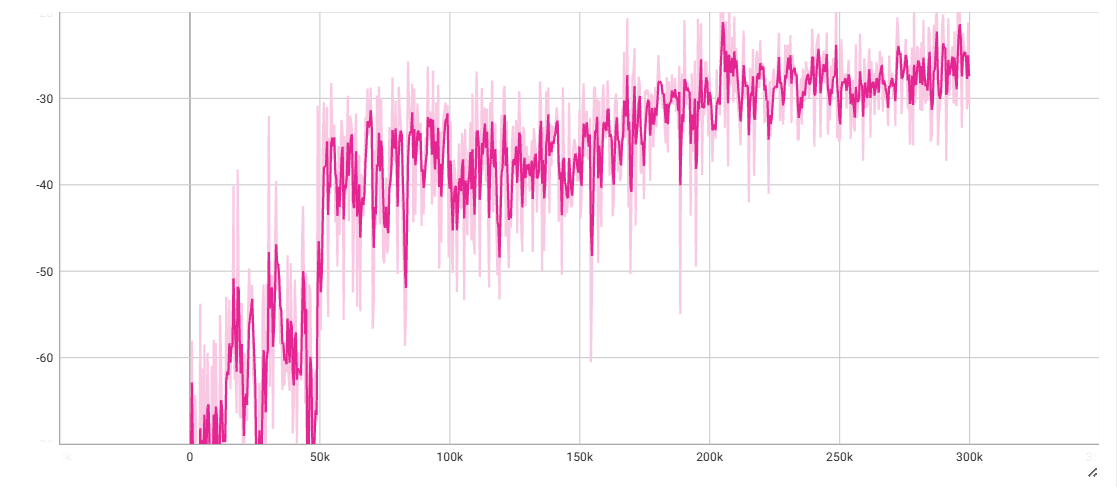
\includegraphics[width=0.41\textwidth]{figuras/reward_base_imagenes.png}
    \caption{Evolución de la recompensa durante el entrenamiento usando únicamente observaciones visuales. La curva permanece en valores negativos y no muestra evidencia clara de resolución de la tarea.}
    \label{fig:reward_base}
\end{figure}

Posteriormente decidimos implementar un enfoque hibrido usando también las observaciones tabulares como parte del input. Esta decisión lleva a una mejora clara de los resultados, principalmente porque la adición de las posiciones guía el aprendizaje y aporta la estructura 3D del entorno.

De manera complementaria, para justificar el uso de las imágenes como input realizamos un estudio de los saliency maps. En el report mostramos el episodio 2 de evaluación, seleccionado por ser representativo del comportamiento del agente y por ofrecer una visualización especialmente clara de la atención del modelo sobre el actuador, el objeto y la región objetivo.

\begin{figure}[H]
    \centering
    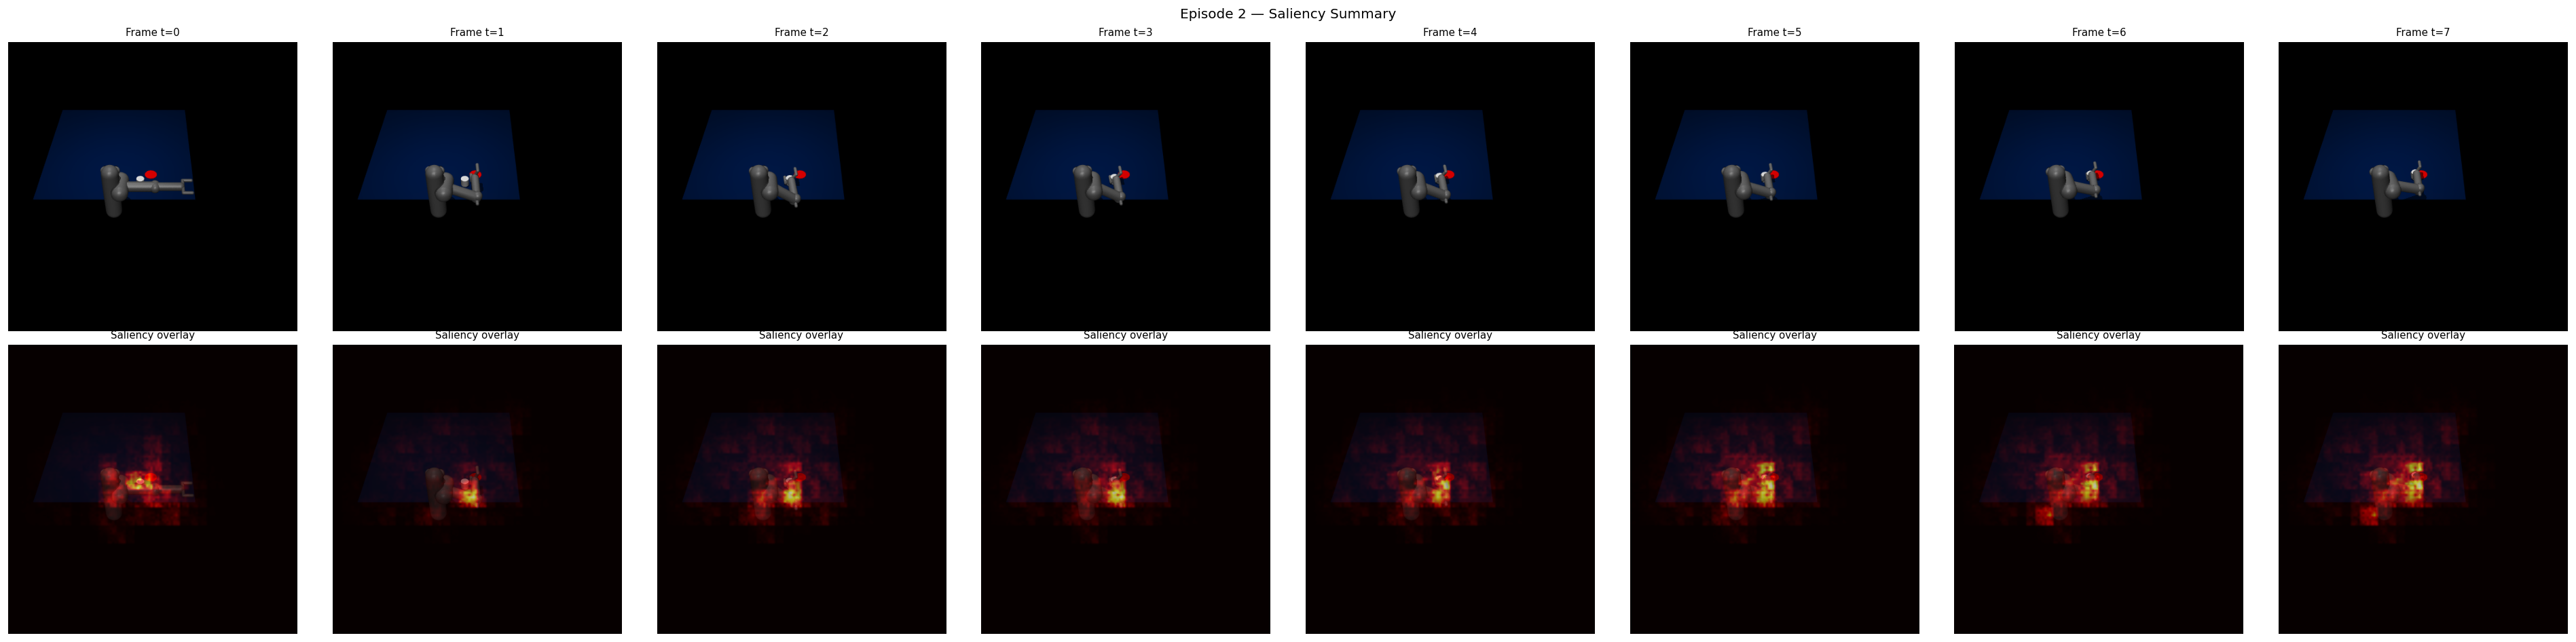
\includegraphics[width=0.41\textwidth]{figuras/ep02_saliency_summary.png}
    \caption{Resumen del análisis de saliency en el episodio 2 de evaluación. La atención del modelo se concentra principalmente en la zona de interacción entre actuador, objeto y objetivo.}
    \label{fig:saliency}
\end{figure}

Como se puede observar en la Figura \ref{fig:saliency}, el agente utiliza de manera efectiva la información visual para tomar decisiones. La atención del modelo se concentra en el actuador, el objeto y el objetivo, lo que indica que la red aprende a extraer de las imágenes los elementos relevantes de la tarea y a combinarlos con las observaciones tabulares para guiar la política.

Esta visualización también permite comprobar que la red no se limita a explotar artefactos visuales irrelevantes, sino que centra buena parte de la señal en elementos funcionalmente importantes para la tarea.

Los resultados del experimento principal muestran que el agente es capaz de aprender una política claramente mejor que la obtenida con solo imágenes tras varios cientos de miles de pasos de entrenamiento. Aunque la curva de recompensa sigue presentando oscilaciones, se observa una mejora sostenida del rendimiento y una mayor capacidad del agente para aproximarse al objeto y empujarlo hacia la meta.

\begin{figure}[H]
    \centering
    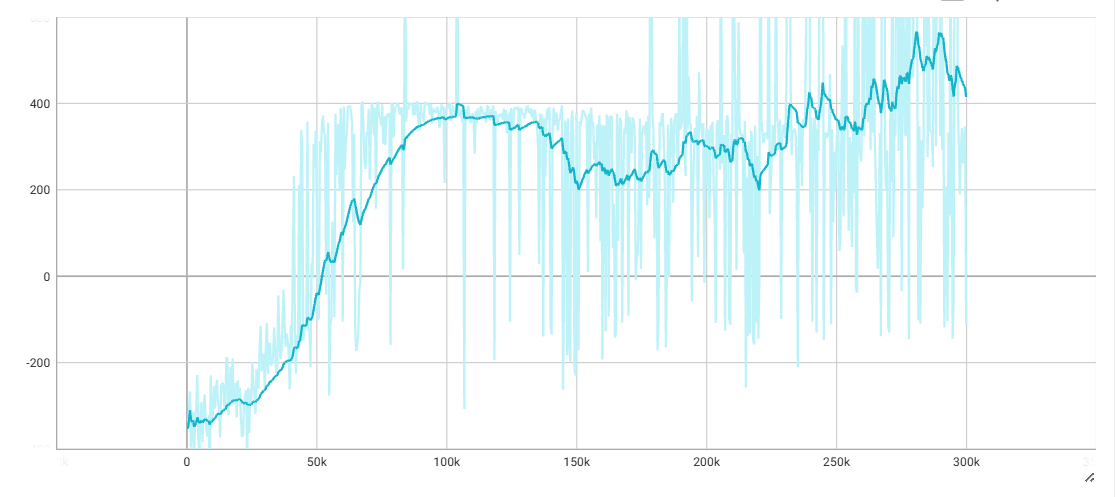
\includegraphics[width=0.41\textwidth]{figuras/reward_final.png}
    \caption{Evolución de la recompensa durante el entrenamiento del modelo híbrido RGB + propiocepción. Se observa una mejora clara con respecto al caso solo visual, aunque persisten oscilaciones en la dinámica de aprendizaje.}
    \label{fig:reward_final}
\end{figure}

De forma complementaria a la evolución de la recompensa, el análisis cualitativo del comportamiento del agente muestra una transición clara desde movimientos aleatorios hacia trayectorias más coordinadas. En las primeras fases del entrenamiento, el actuador no mantiene una estrategia consistente y con frecuencia no alcanza el objeto. Sin embargo, conforme avanza el aprendizaje, el brazo comienza a aproximarse con mayor precisión, estableciendo contacto con el objeto y generando empujes más dirigidos hacia la región objetivo.

Este comportamiento sugiere que la política aprendida no solo mejora en términos de recompensa acumulada, sino también en términos de estructura del comportamiento. En un entorno de manipulación como \texttt{Pusher-v5}, esta transición resulta especialmente importante, ya que el éxito requiere coordinar varias subtareas consecutivas.

Adicionalmente, los episodios de evaluación permiten analizar de forma cualitativa la política aprendida. En las ejecuciones finales se observa que el agente no solo incrementa la recompensa acumulada, sino que desarrolla una secuencia de acciones más coherente: aproximación al objeto, contacto y empuje progresivo hacia la meta.

\begin{figure}[H]
    \centering
    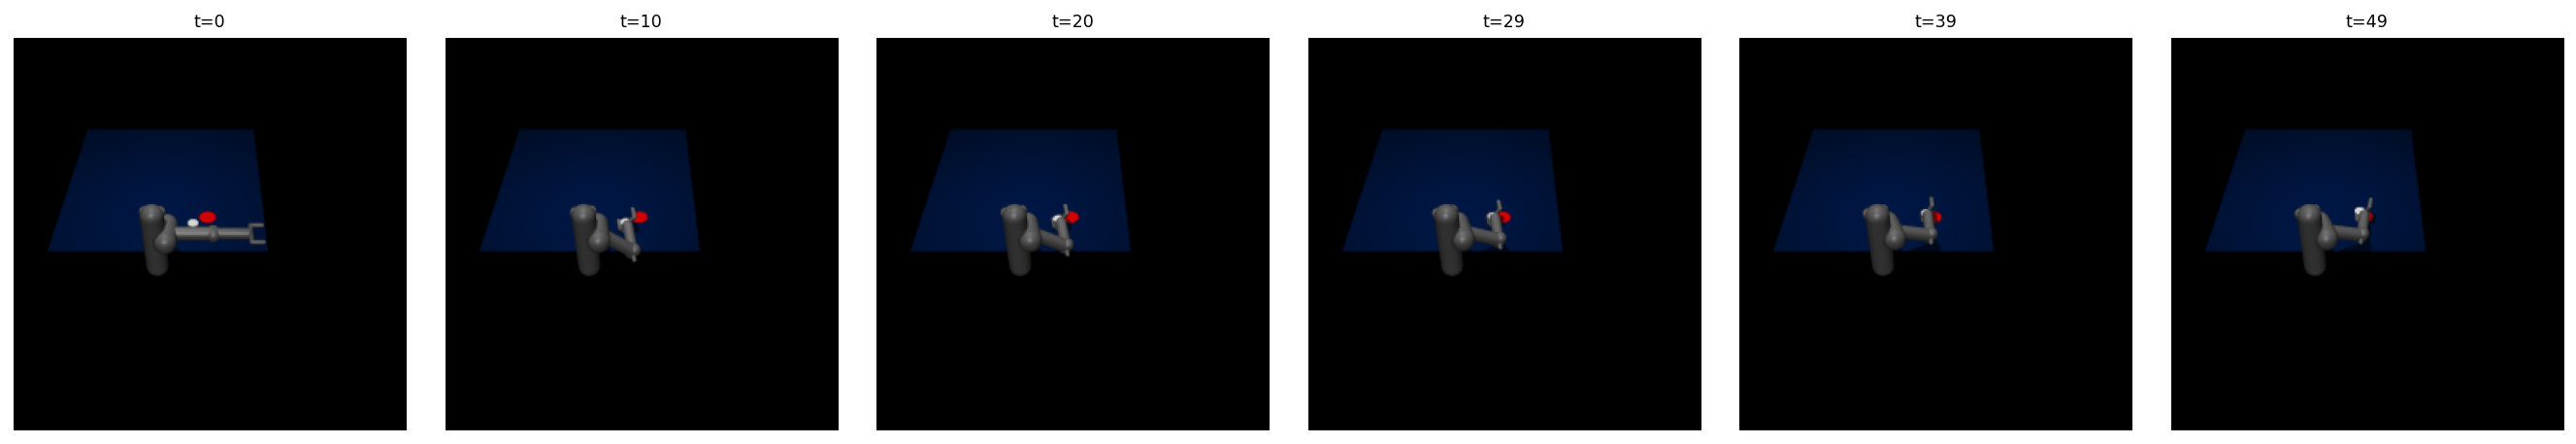
\includegraphics[width=0.43\textwidth]{figuras/rollout_frames_ep02.png}
    \caption{Secuencia de frames extraída del episodio 2 de evaluación. Se observa una política más estructurada, con fases de aproximación al objeto y empuje hacia la región objetivo.}
    \label{fig:rollout_frames}
\end{figure}

\subsection{Conclusiones de la Parte 1}

Los resultados obtenidos permiten concluir que al incorporar información tabular de las posiciones del robot, el objeto y el objetivo junto con las observaciones visuales mejora de forma significativa el rendimiento del agente, ya que proporciona una representación estructurada del estado del sistema que complementa la información visual. Este enfoque híbrido facilita el aprendizaje de la dinámica del entorno y acelera la convergencia hacia políticas útiles.

Adicionalmente, el análisis de saliency maps confirma que la red neuronal es capaz de centrar su atención en las regiones relevantes de la imagen, como el efector del robot, el objeto y el objetivo, lo que valida parcialmente la utilidad del canal visual dentro del modelo. Más aún, las visualizaciones obtenidas muestran que el agente sí aprende de las imágenes: no solo recibe el canal visual como entrada, sino que basa parte de su decisión en la información espacial contenida en él.

\section{Parte 2: Sensibilidad a hiperparámetros}

\subsection{Metodología}

En esta segunda parte del trabajo se realiza un estudio sistemático de la sensibilidad del algoritmo SAC frente a distintos hiperparámetros relevantes. Para ello se ha implementado un esquema de \textit{grid search} que permite evaluar múltiples configuraciones de forma automática, manteniendo una estructura experimental controlada y reproducible.

El espacio de búsqueda incluye parámetros críticos del algoritmo como la tasa de aprendizaje, el tamaño del batch, la arquitectura del extractor de características y los parámetros relacionados con el aprendizaje del curriculum. Hemos centrado el estudio en la tasa de aprendizaje, el tamaño de salida del mlp que recibe como input los datos tabulares y el tamaño de las imagenes para estudiar el impacto de cada tipo de entrada. Cada combinación de hiperparámetros se entrena de forma independiente durante un número fijo de pasos.

El entorno utilizado es exactamente el mismo que en la Parte 1, manteniendo la arquitectura multimodal de observación (imágenes RGB y features propioceptivas), así como el esquema de recompensa basado en curriculum learning. De esta forma, se asegura que las variaciones observadas en el rendimiento se deban exclusivamente a cambios en los hiperparámetros y no a diferencias en la configuración del entorno.

\subsection{Resultados y discusión}

Los resultados del grid search muestran que el rendimiento del agente es altamente sensible a ciertos hiperparámetros clave del algoritmo SAC. En la Figura \ref{fig:grid_comparison} se pueden observar los resultados generales obtenidos.

\begin{figure}[H]
    \centering
    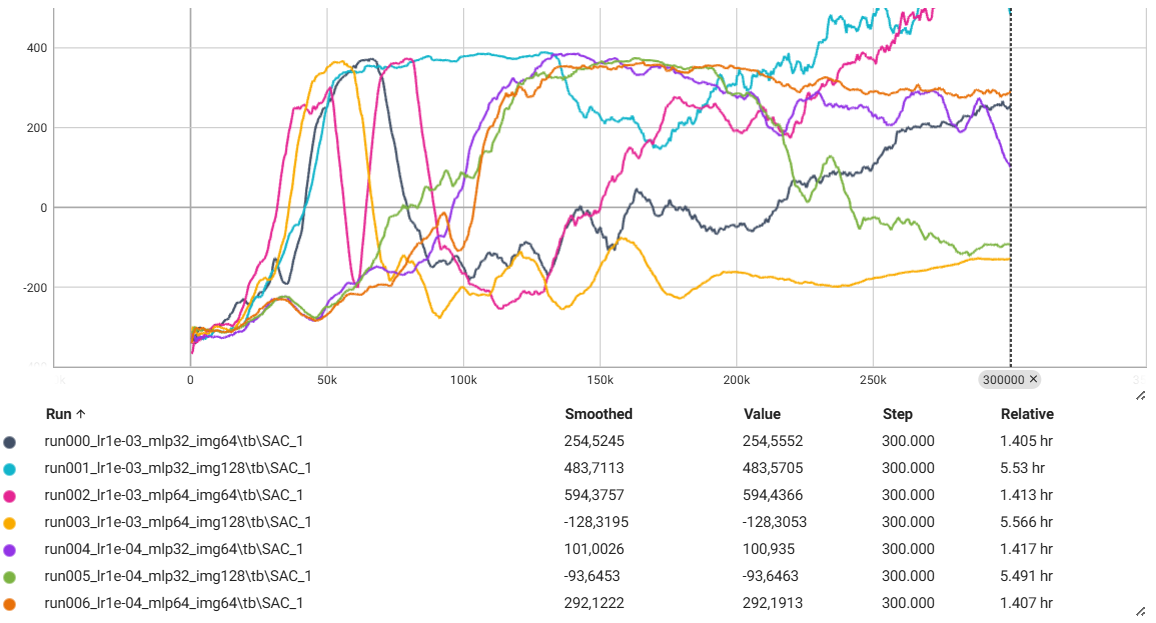
\includegraphics[width=0.41\textwidth]{figuras/grid_comparison.png}
    \caption{Comparación global de las configuraciones evaluadas en el grid search. Se observan diferencias importantes tanto en recompensa final como en coste temporal entre configuraciones.}
    \label{fig:grid_comparison}
\end{figure}

La tasa de aprendizaje tiene un impacto significativo en la dinámica de entrenamiento. En las configuraciones evaluadas, \(1\times10^{-3}\) puede alcanzar las mejores recompensas finales, pero también produce trayectorias más inestables y mayor sensibilidad al resto de hiperparámetros. Por su parte, \(1\times10^{-4}\) tiende a mostrar una evolución más conservadora y, en algunos casos, más consistente, aunque no siempre alcanza el mejor rendimiento final.

\begin{figure}[H]
    \centering
    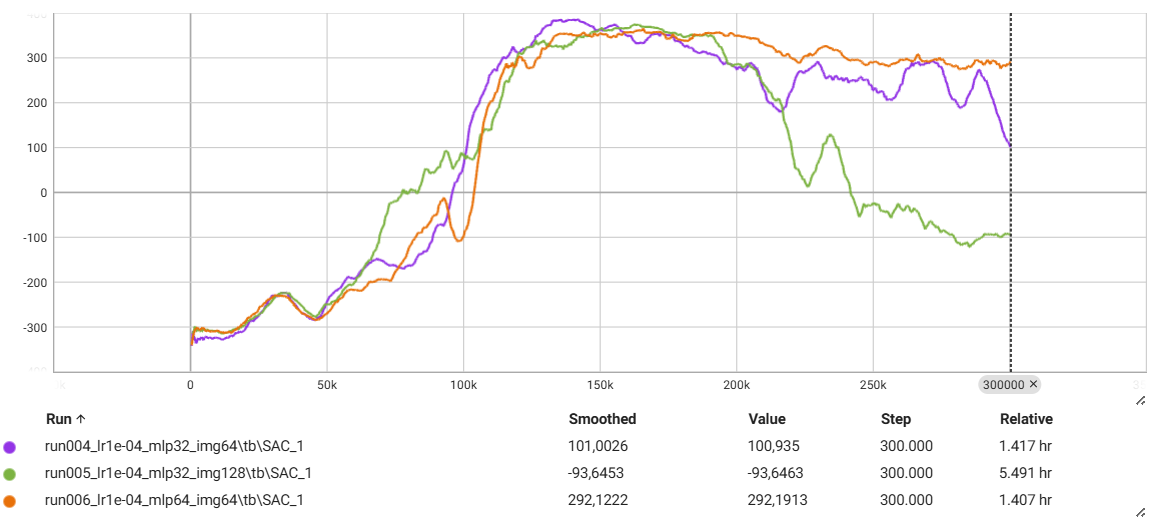
\includegraphics[width=0.41\textwidth]{figuras/grid_lr4.png}
    \caption{Comparación de runs con learning rate \(1\times10^{-4}\). La evolución es en general más conservadora, aunque el rendimiento final depende de la combinación con el resto de hiperparámetros.}
    \label{fig:grid_lr4}
\end{figure}

En comparación, como se puede observar en las Figuras \ref{fig:grid_lr3} y \ref{fig:grid_lr4}, no existe una única conclusión simple sobre la mejor tasa de aprendizaje. Más bien, los resultados sugieren una interacción importante entre learning rate, resolución de imagen y tamaño de la rama tabular. Esto refuerza la idea de que el rendimiento de SAC depende de combinaciones de hiperparámetros y no de un único parámetro aislado.

\begin{figure}[H]
    \centering
    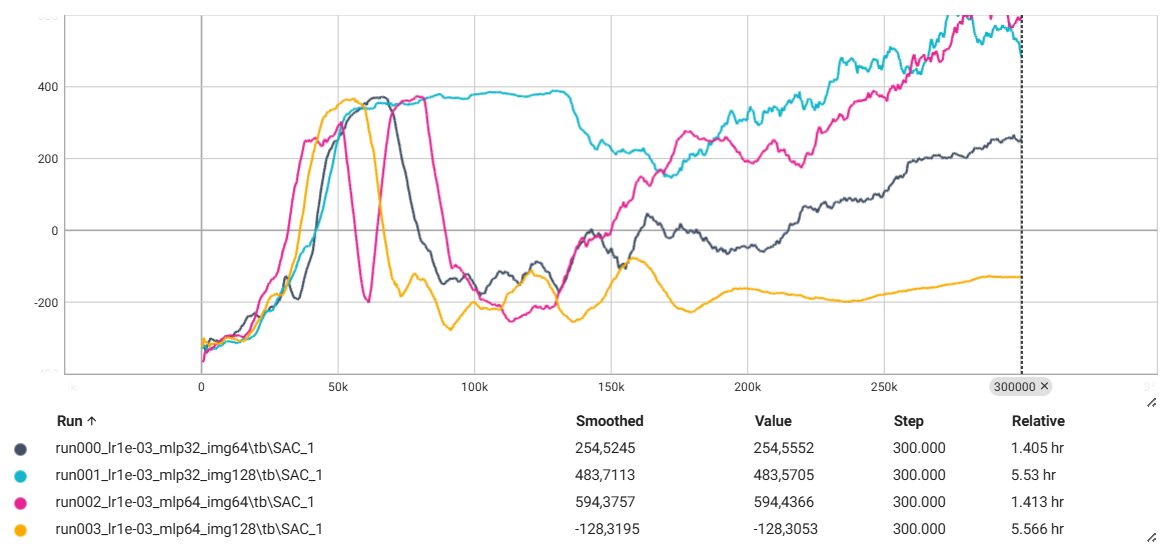
\includegraphics[width=0.41\textwidth]{figuras/grid_lr3.png}
    \caption{Comparación de runs con learning rate \(1\times10^{-3}\). Esta tasa permite alcanzar algunas de las mejores recompensas finales, pero también presenta trayectorias más inestables.}
    \label{fig:grid_lr3}
\end{figure}

En cuanto a la arquitectura del extractor de características, se observa que el tamaño de la representación latente (dimensiones de salida de la CNN y del MLP) influye en la capacidad de representación del modelo. Representaciones demasiado pequeñas limitan la expresividad del modelo, mientras que representaciones demasiado grandes no aportan mejoras significativas y aumentan el coste computacional.

\begin{figure}[H]
    \centering
    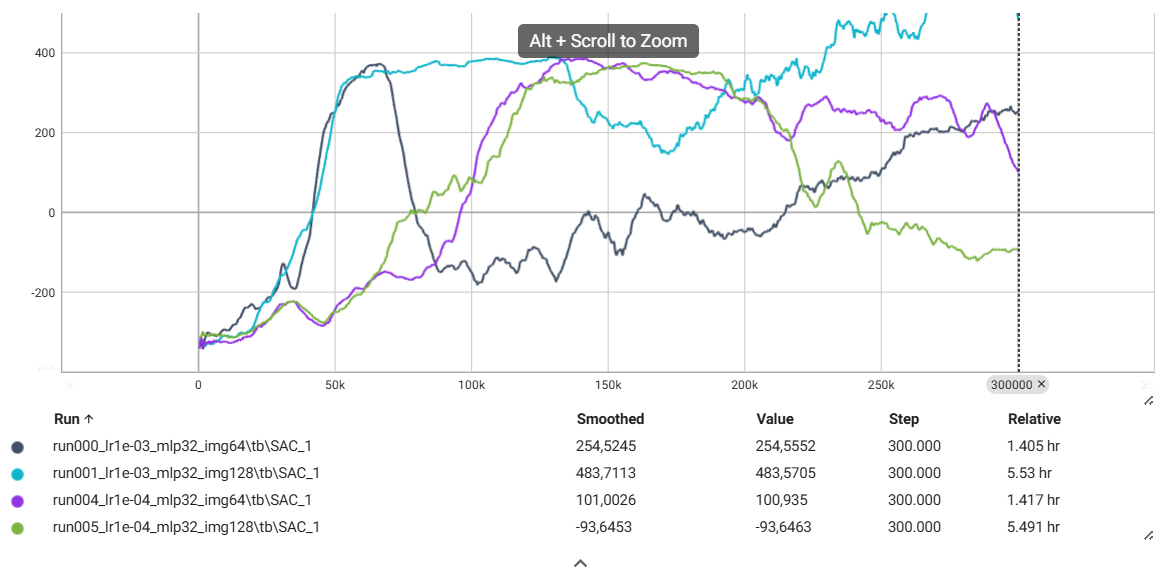
\includegraphics[width=0.41\textwidth]{figuras/grid_mlp32.png}
    \caption{Runs con dimensión de salida MLP igual a 32. El rendimiento depende también del learning rate y de la resolución empleada.}
    \label{fig:grid_mlp32}
\end{figure}

\begin{figure}[H]
    \centering
    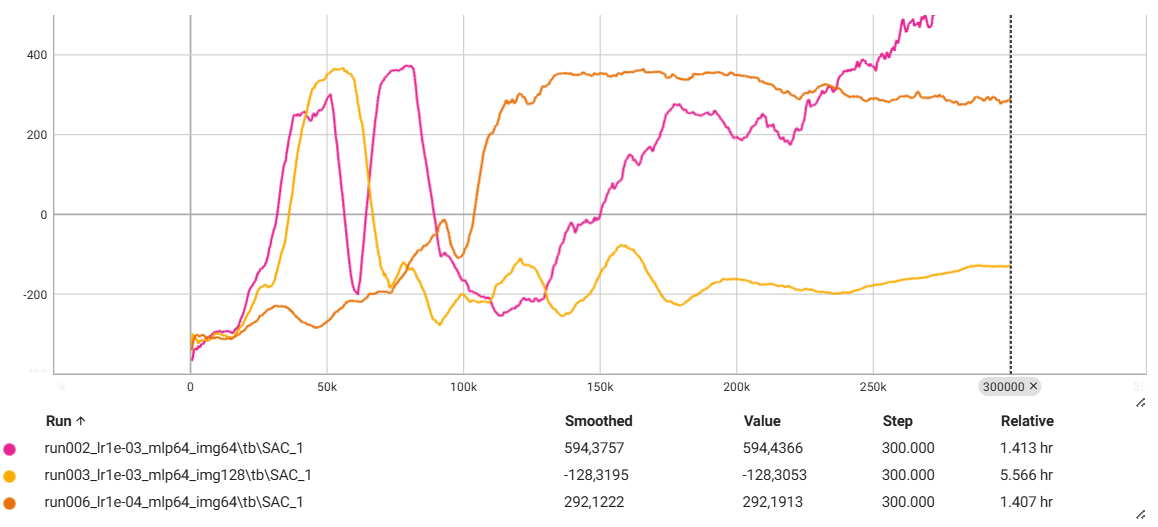
\includegraphics[width=0.41\textwidth]{figuras/grid_mlp64.png}
    \caption{Runs con dimensión de salida MLP igual a 64. Algunas configuraciones alcanzan las mejores recompensas finales del estudio, aunque con variabilidad entre ejecuciones.}
    \label{fig:grid_mlp64}
\end{figure}

Como se puede ver en las Figuras \ref{fig:grid_mlp32} y \ref{fig:grid_mlp64}, el tamaño de la rama MLP influye en el rendimiento, pero su efecto es menos claro y menos dominante que el de la resolución de imagen. En particular, algunas configuraciones con \texttt{mlp\_output\_dim}=64 alcanzan recompensas superiores, aunque también mantienen una variabilidad apreciable entre ejecuciones.

\begin{figure}[H]
    \centering
    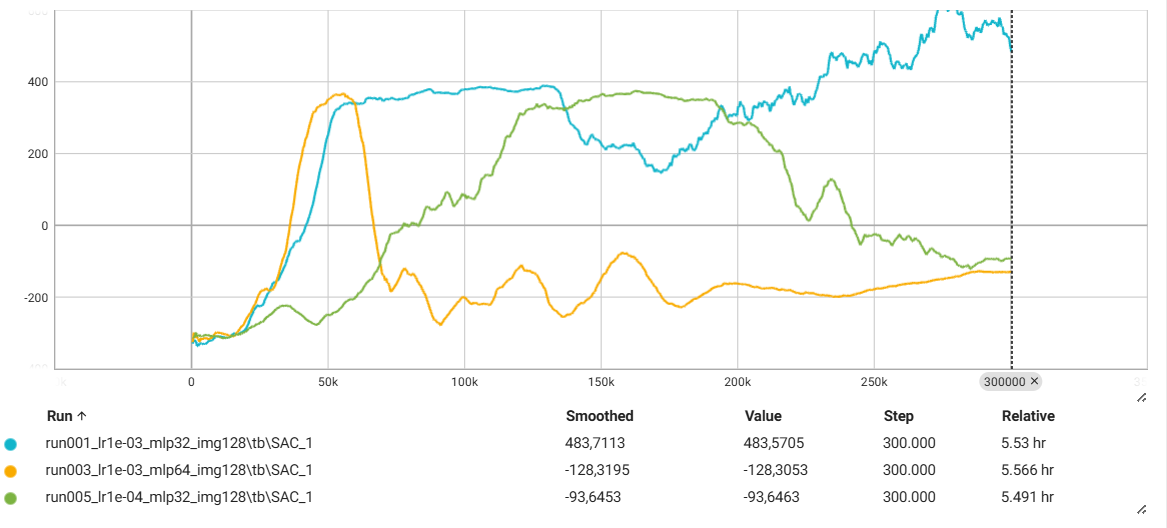
\includegraphics[width=0.41\textwidth]{figuras/grid_img128.png}
    \caption{Runs con resolución de entrada \(128\times128\). Se observa un mayor coste computacional y, en general, peores resultados que con \(64\times64\).}
    \label{fig:grid_img128}
\end{figure}

\begin{figure}[H]
    \centering
    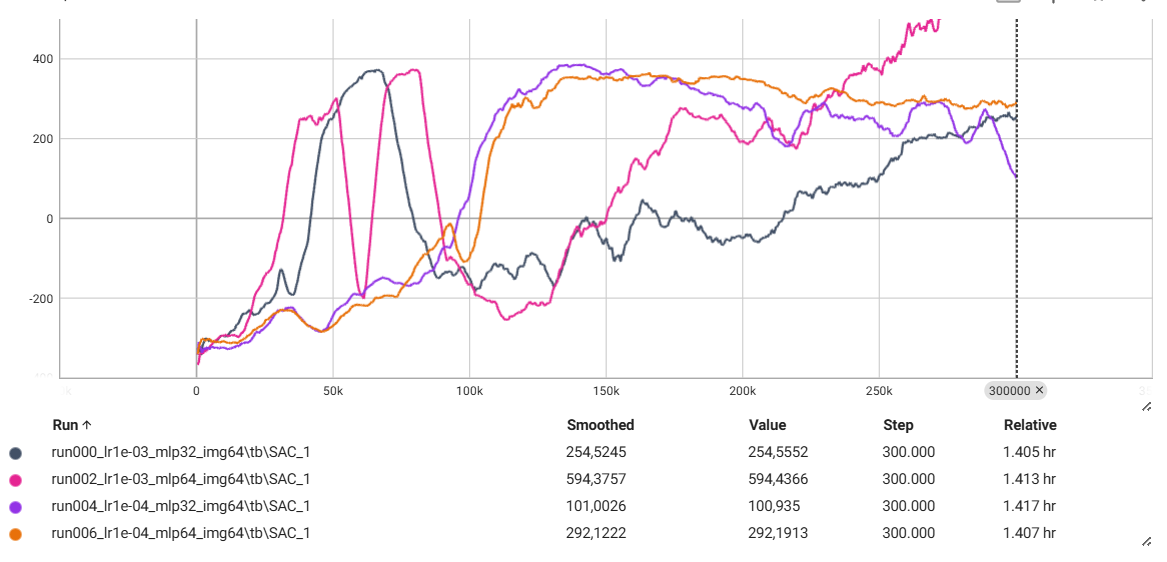
\includegraphics[width=0.41\textwidth]{figuras/grid_img64.png}
    \caption{Runs con resolución de entrada \(64\times64\). Estas configuraciones muestran, en conjunto, mejores recompensas y mayor eficiencia computacional.}
    \label{fig:grid_img64}
\end{figure}

Mientras tanto, se observa claramente en las Figuras \ref{fig:grid_img128} y \ref{fig:grid_img64} que el tamaño de la imagen influye de manera muy significativa tanto en el rendimiento como en el coste computacional. Las configuraciones con imágenes de \(64\times64\) alcanzan, en general, mejores recompensas y una evolución más favorable que las de \(128\times128\). Además, las ejecuciones con mayor resolución requieren aproximadamente cuatro veces más tiempo de entrenamiento, lo que refuerza la idea de que aumentar la resolución no resulta rentable en este entorno bajo las restricciones computacionales de la práctica.

Los resultados globales del grid search confirman que existe un conjunto reducido de configuraciones óptimas que equilibran rendimiento y estabilidad, mientras que la mayoría de combinaciones producen políticas subóptimas o inestables.

\begin{table}[H]
\centering
\caption{Resumen cualitativo de tendencias observadas en el grid search.}
\label{tab:grid_trends}
\begin{tabular}{p{3.0cm}p{3.8cm}}
\toprule
Factor & Tendencia observada \\
\midrule
Resolución de imagen & \(64\times64\) supera generalmente a \(128\times128\) en rendimiento y coste computacional. \\
Learning rate & \(10^{-3}\) alcanza las mejores runs, pero con mayor inestabilidad; \(10^{-4}\) muestra una evolución más conservadora. \\
Dimensión MLP & El efecto existe, pero es menos dominante que el de la resolución de imagen. \\
Canal visual & Aporta información relevante, pero no resulta suficiente por sí solo. \\
\bottomrule
\end{tabular}
\end{table}

\subsubsection{Análisis de eficiencia computacional}

Además del rendimiento medido en recompensa, el estudio de hiperparámetros permite analizar el coste computacional asociado a cada configuración. En particular, la resolución de entrada tiene un impacto muy relevante sobre el tiempo total de entrenamiento. Las configuraciones con imágenes de mayor tamaño requieren más memoria y aumentan el coste del paso hacia delante y hacia atrás de la red convolucional.

Esto hace que, incluso cuando la mejora en recompensa es pequeña o inexistente, el coste temporal de aumentar la resolución sea muy elevado. Desde el punto de vista práctico, este resultado refuerza la idea de que no siempre una representación visual de mayor calidad implica un mejor aprendizaje, especialmente cuando el agente dispone además de información propioceptiva.

\begin{table}[H]
\centering
\caption{Coste computacional medio por resolución de imagen.}
\label{tab:cost_by_resolution}
\begin{tabular}{lcc}
\toprule
Resolución & Tiempo medio (h) & Reward medio \\
\midrule
$64\times64$ & 1.41 $\pm$ 0.00 & 439.3 \\
$128\times128$ & 5.53 $\pm$ 0.03 & -156.4 \\
\bottomrule
\end{tabular}
\end{table}

La Tabla \ref{tab:cost_by_resolution} cuantifica de forma directa el impacto de la resolución sobre el coste de entrenamiento. Las configuraciones con imágenes de \(128\times128\) requieren aproximadamente cuatro veces más tiempo que las de \(64\times64\), y además obtienen peores recompensas medias. Este resultado refuerza la idea de que, en este entorno, aumentar la resolución no compensa ni en rendimiento ni en eficiencia.

\subsubsection{Análisis de variabilidad}

Otro aspecto relevante de los experimentos es la variabilidad entre configuraciones y entre ejecuciones. Aunque el grid search permite identificar tendencias generales, también se observa que pequeñas modificaciones en los hiperparámetros pueden generar trayectorias de aprendizaje muy distintas.

Esta sensibilidad es habitual en Deep Reinforcement Learning, especialmente en tareas de control continuo con representación visual. En consecuencia, los resultados deben interpretarse no solo en términos de la mejor configuración puntual, sino también considerando la robustez y estabilidad de cada elección de hiperparámetros.

\begin{table}[H]
\centering
\caption{Resumen de configuraciones destacadas del grid search.}
\label{tab:grid_best_worst_stable}
\begin{tabular}{p{2.0cm}p{4.0cm}}
\toprule
Categoría & Configuración \\
\midrule
Mejor run & run002\_lr1e-03\_mlp64\_img64 (reward=1155.3, std=220.3) \\
Peor run & run003\_lr1e-03\_mlp64\_img128 (reward=-298.5, std=53.5) \\
Más estable & run006\_lr1e-04\_mlp64\_img64 (reward=395.0, std=7.5) \\
\bottomrule
\end{tabular}
\end{table}

La Tabla \ref{tab:grid_best_worst_stable} resume tres configuraciones representativas del estudio: la mejor run en recompensa final, la peor configuración y la más estable en términos de varianza. Esto permite distinguir entre configuraciones que maximizan rendimiento y configuraciones que, sin ser las mejores, ofrecen un comportamiento más robusto y reproducible.

\subsection{Conclusiones de la Parte 2}

El estudio de sensibilidad a hiperparámetros permite concluir que el rendimiento del algoritmo SAC en tareas de manipulación robótica es altamente dependiente de la configuración del entrenamiento.

En particular, la resolución de imagen emerge como uno de los factores más determinantes, mientras que la tasa de aprendizaje condiciona fuertemente la estabilidad y el potencial de rendimiento final.

Este análisis confirma la importancia de una correcta selección de hiperparámetros en problemas de control continuo con observaciones de alta dimensionalidad. Además, pone de manifiesto que el diseño manual de estos parámetros puede resultar costoso, lo que motiva el uso de técnicas más avanzadas de optimización automática de hiperparámetros en futuros trabajos.

\section{Parte 3: Estudio de ablación}

\subsection{Motivación}

Aunque en las secciones anteriores se ha observado que el enfoque multimodal junto con el uso de curriculum learning permite obtener políticas razonables, todavía no está claro qué componentes del sistema son realmente los responsables de esta mejora. Es decir, no basta con comprobar que el modelo completo funciona, sino que también es necesario entender qué aporta cada una de sus partes.

Con este objetivo, se planteó un estudio de ablación en el que se analizó por separado tres elementos clave del proyecto: el uso del reward shaping basado en curriculum, la información tabular propioceptiva y la información visual. Este análisis permite estudiar hasta qué punto el rendimiento final depende de cada uno de estos factores y si realmente todos ellos son necesarios.

\subsection{Configuración experimental}

Para que la comparación sea lo más limpia y justa posible, todas las variantes se entrenan manteniendo los mismos hiperparámetros y el mismo entorno, modificando únicamente los componentes que se quieren analizar.

En concreto, se consideran las siguientes configuraciones:

\begin{itemize}
    \item \textbf{Multimodal con curriculum}: modelo completo, que utiliza imágenes, features tabulares y reward shaping progresivo durante el entrenamiento.
    \item \textbf{Multimodal sin curriculum}: misma arquitectura multimodal, pero entrenada directamente con la recompensa original del entorno.
    \item \textbf{Solo features}: el agente recibe únicamente observaciones tabulares y se entrena con la recompensa original.
    \item \textbf{Solo imágenes}: el agente recibe únicamente observaciones visuales y se entrena con la recompensa original.
\end{itemize}

Todas las variantes se entrenan durante 300\,000 pasos. Para poder comparar los resultados de forma consistente, todas las políticas se evalúan utilizando una misma recompensa común, es decir, la recompensa original del entorno, independientemente de la función de recompensa empleada durante el entrenamiento.

\subsection{Resultados y discusión}

Para analizar los resultados no se ha considerado solo la recompensa final, sino también su evolución a lo largo del entrenamiento. Esto permite ver mejor cómo aprende cada modelo, si lo hace de forma estable y si la mejora es progresiva o depende de momentos concretos.

\begin{figure}[H]
    \centering
    \includegraphics[width=0.43\textwidth]{figuras/ablation_eval_and_training.png}
    \caption{Arriba: recompensa media de evaluación durante el entrenamiento para cada variante. Abajo: recompensa media por episodio durante el entrenamiento.}
    \label{fig:ablation_curves}
\end{figure}

En la parte superior de la Figura \ref{fig:ablation_curves} se ve la recompensa de evaluación, que es la métrica más importante para comparar las distintas configuraciones. Se observa claramente que la variante \textit{multimodal sin curriculum} es la que mejor rinde durante casi todo el entrenamiento. Además, su curva es bastante estable, con pocas oscilaciones, lo que sugiere un aprendizaje robusto.

La variante \textit{solo features} se sitúa en segundo lugar. Aunque no llega al nivel de la mejor configuración, su rendimiento es razonable y mejora claramente al de solo imágenes. Esto sugiere que la información tabular es la parte más necesaria para resolver la tarea.

La variante \textit{multimodal con curriculum} tiene un comportamiento más irregular. En algunos tramos se acerca a \textit{solo features}, pero no logra superarla al final y termina ligeramente por debajo. Además, la curva oscila más, lo que indica una mayor inestabilidad.

Por último, la variante \textit{solo imágenes} queda claramente por debajo del resto durante todo el entrenamiento. Apenas muestra una mejora apreciable, lo que indica que, en las condiciones de esta práctica, la información visual por sí sola no es suficiente para aprender una política útil, aunque eso no significa que no aporte al aprendizaje en la parte multimodal.

La parte inferior de la figura muestra la recompensa de entrenamiento, y aquí aparece un resultado interesante. La variante \textit{solo features} alcanza valores muy altos, incluso mejores que los del modelo multimodal. Sin embargo, esa ventaja no se traduce del todo en la evaluación final. Algo parecido ocurre con la variante \textit{multimodal con curriculum}, que también logra recompensas de entrenamiento altas pero no obtiene el mejor rendimiento en evaluación.

En cambio, la variante \textit{multimodal sin curriculum}, que es la mejor en evaluación, presenta valores de recompensa de entrenamiento más modestos y bastante planos. Esto sugiere que optimizar más la reward durante el entrenamiento no implica necesariamente obtener una mejor política final cuando se evalúa con una métrica común.

Este resultado es especialmente relevante. En las variantes con curriculum, el agente se entrena utilizando una función de recompensa modificada que enfatiza subtareas intermedias, como la aproximación al objeto o el contacto inicial. Este diseño facilita la exploración y permite alcanzar recompensas más altas durante el entrenamiento.

Sin embargo, en la fase de evaluación todas las configuraciones se comparan utilizando la recompensa original del entorno, sin aplicar dicho shaping. Como consecuencia, las políticas entrenadas con curriculum no están necesariamente optimizadas para esta métrica final, ya que han sido guiadas por una señal de aprendizaje distinta.

Esto explica por qué la variante \textit{multimodal sin curriculum} obtiene mejores resultados en evaluación, a pesar de que durante el entrenamiento el curriculum produce recompensas más altas y comportamientos más estructurados. En este sentido, el resultado no implica que el curriculum sea perjudicial, sino que pone de manifiesto una desalineación entre la función de entrenamiento y la métrica de evaluación.

Para completar el análisis, en la Figura \ref{fig:ablation} se muestra un resumen de la evaluación final de cada variante. Esta figura confirma lo observado en las curvas: bajo la métrica de evaluación utilizada, la mejor configuración es la multimodal sin curriculum, seguida de la variante solo features, mientras que usar únicamente imágenes produce los peores resultados.

\begin{figure}[H]
    \centering
    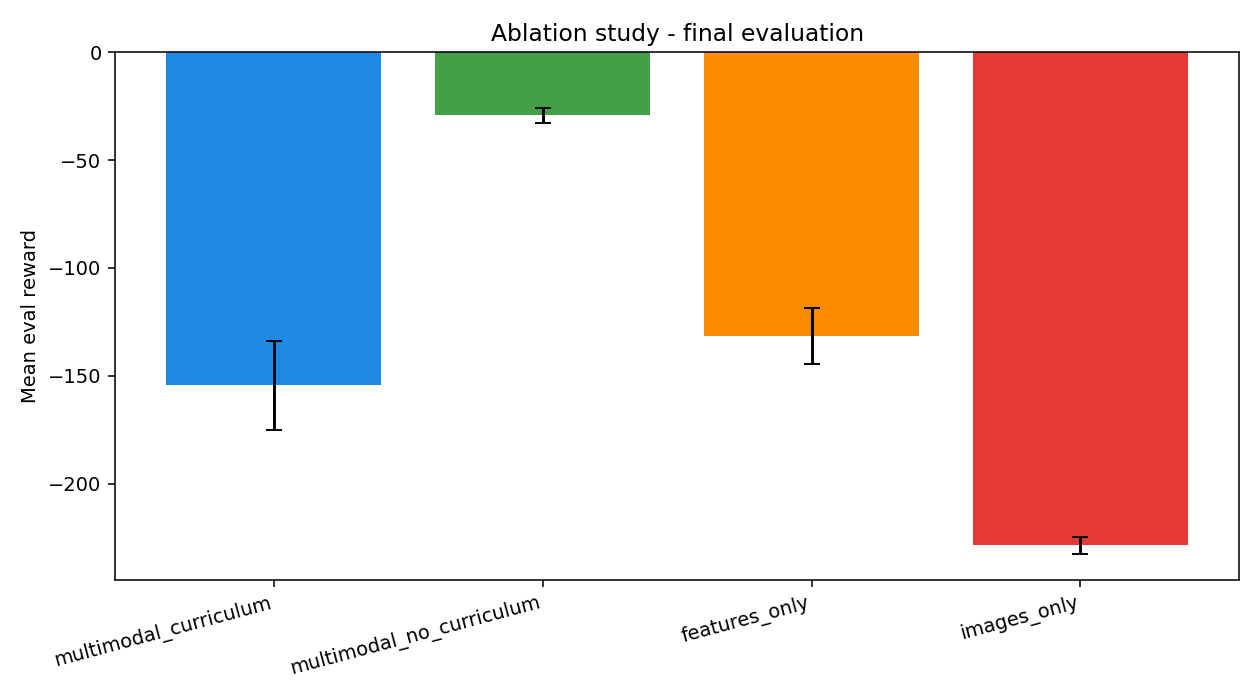
\includegraphics[width=0.41\textwidth]{figuras/ablation_comparison.png}
    \caption{Recompensa media de evaluación final para cada variante del estudio de ablación.}
    \label{fig:ablation}
\end{figure}

\subsection{Conclusiones de la Parte 3}

El estudio de ablación permite extraer varias conclusiones importantes. En primer lugar, la información tabular es fundamental para el aprendizaje de la tarea, ya que incluso sin la parte visual el agente es capaz de aprender políticas razonables. En segundo lugar, el uso exclusivo de imágenes no es suficiente bajo las limitaciones de resolución y computación de esta práctica; quizá con más pasos podría mejorar, pero con 300k \textit{steps} sigue estando muy lejos del resto de configuraciones.

Por otro lado, la combinación multimodal sí aporta beneficios. Sin embargo, el uso de curriculum learning en la recompensa no mejora el rendimiento final bajo la métrica de evaluación utilizada. En concreto, la mejor configuración en evaluación es la multimodal sin curriculum.

Este resultado debe interpretarse con cuidado, ya que las variantes con curriculum se entrenan con una función de recompensa distinta a la utilizada en evaluación. Como se ha visto, el curriculum permite obtener recompensas de entrenamiento más altas y facilita la exploración, pero su señal no está completamente alineada con la métrica final. Esto puede hacer que las políticas aprendidas no se traduzcan directamente en mejores resultados bajo la recompensa original.

Finalmente, el análisis conjunto de la recompensa de entrenamiento y de evaluación pone de manifiesto que ambas no siempre cuentan la misma historia. Algunas configuraciones optimizan muy bien la reward interna del entrenamiento, pero no generan las mejores políticas cuando se evalúan con una métrica común. Esto refuerza la importancia de analizar no solo el valor final de la recompensa, sino también la dinámica de aprendizaje y la coherencia entre las distintas métricas.

\section{Conclusión general}

A lo largo de este trabajo se ha estudiado el comportamiento de SAC en una tarea de manipulación robótica continua dentro del entorno \texttt{Pusher-v5}. Los resultados obtenidos muestran que el algoritmo es capaz de aprender políticas útiles, pero también que su rendimiento depende en gran medida de cómo se representa el estado, de cómo se diseña la recompensa y de cómo se ajustan los hiperparámetros del entrenamiento.

En primer lugar, se ha comprobado que el uso exclusivo de imágenes no es suficiente para aprender una política estable bajo las restricciones de resolución y coste computacional de esta práctica. En cambio, la incorporación de información tabular propioceptiva mejora claramente el aprendizaje y permite al agente explotar de forma más eficaz la estructura de la tarea. Al mismo tiempo, el análisis de saliency maps muestra que el canal visual sí aporta información relevante, ya que la red centra su atención en el actuador, el objeto y la meta.

En segundo lugar, el estudio de sensibilidad a hiperparámetros confirma que pequeñas variaciones en parámetros como la tasa de aprendizaje o la resolución de entrada pueden producir comportamientos muy distintos. En particular, las configuraciones con imágenes de \(64\times64\) han resultado más eficientes y, en conjunto, más efectivas que las de \(128\times128\), lo que pone de manifiesto la importancia de equilibrar calidad de representación y coste de entrenamiento.

Por último, el estudio de ablación ha permitido entender mejor qué componentes explican realmente la mejora del sistema. Los resultados muestran que la información tabular desempeña un papel fundamental, que el uso exclusivo de imágenes produce los peores resultados y que, en esta implementación concreta, la variante multimodal sin curriculum alcanza el mejor rendimiento final bajo la métrica de evaluación utilizada.

Este resultado no implica que el curriculum learning sea perjudicial, sino que pone de manifiesto la importancia de la alineación entre la función de recompensa utilizada durante el entrenamiento y la métrica de evaluación final. En este caso, el curriculum facilita el aprendizaje y mejora la dinámica de entrenamiento, pero su señal no coincide completamente con la recompensa empleada en evaluación, lo que limita su impacto en los resultados finales.

\section*{Trabajo futuro}

Como líneas futuras se propone:
\begin{itemize}
    \item Aplicar SAC directamente en entornos de manipulación (por ejemplo, tareas de empuje).
    \item Explorar representaciones basadas unicamente en imágenes.
    \item Incorporar técnicas de aprendizaje por demostración.
    \item Evaluar variantes más recientes como SACv2 o métodos híbridos.
\end{itemize}

\end{document}